% F16 Predicted Anny age per Relative Human group (adult, teen, kid, baby) for Base and Final, with the child
% threshold 0.45 (Results 6.7). PLACEHOLDER: data pending.
% Waits for (REWRITE_PLAN.md section 3 "F15 and F16, CSVs"; section 7 Q11):
%   data/F16_rh_base.csv    <- results/diagnostics/relative_human_val_anny_s2_shape_v5_00099/per_person.csv
%   data/F16_rh_final.csv   <- results/diagnostics/relative_human_val_exp7_v5_final_00009/per_person.csv
%   data/F16_rh_masked.csv  <- the masked arm's per_person.csv (optional third model)
% Column names known (data/CLUSTER_ANSWERS.md): age_group, pred_age, matched (keep matched rows).
% Then one \addplot[boxplot] table[y=pred_age] per age_group and model (pgfplots statistics library is loaded).
\begin{figure}[tbp]
\centering
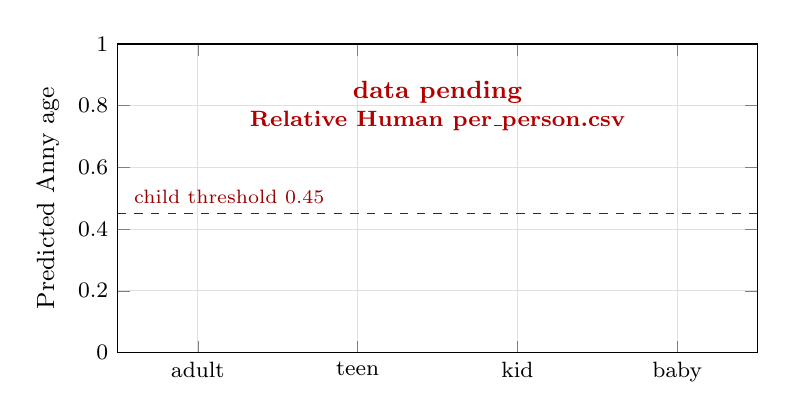
\begin{tikzpicture}
\begin{axis}[
  width=0.8\linewidth, height=5.5cm,
  ylabel={Predicted Anny age}, ymin=0, ymax=1,
  xmin=0.5, xmax=4.5, xtick={1,2,3,4}, xticklabels={adult, teen, kid, baby},
  grid=major, grid style={gray!25},
  tick label style={font=\footnotesize}, label style={font=\small},
]
\draw[dashed, red!60!black] (axis cs:0.5,0.45) -- (axis cs:4.5,0.45) node[pos=0.01, anchor=south west, font=\scriptsize] {child threshold 0.45};
\node[font=\small\bfseries, red!70!black, align=center] at (axis cs:2.5,0.8) {data pending\\[-1pt]\footnotesize Relative Human per\_person.csv};
\end{axis}
\end{tikzpicture}
\caption{Predicted Anny age per Relative Human age group, Base and Final; detected people only. \TODO{plot pending:
Relative Human per-person CSVs}}
\label{fig:rh-age}
\end{figure}
